\section{Camera theory}

An image captured through a camera is the result of reflected light being detected on a camera sensor, see figure \ref{fig:light_cam}. This process is know as \textit{image acquisition}. The process is generally not something one thinks about when capturing an image with a camera, since it all happens automatically. In this section the basics of image acquisition using a digital camera will be explained. In order to understand how this works it is necessary to have a basic understanding of the physics behind light.

\begin{figure}[htbp] 
\centering 
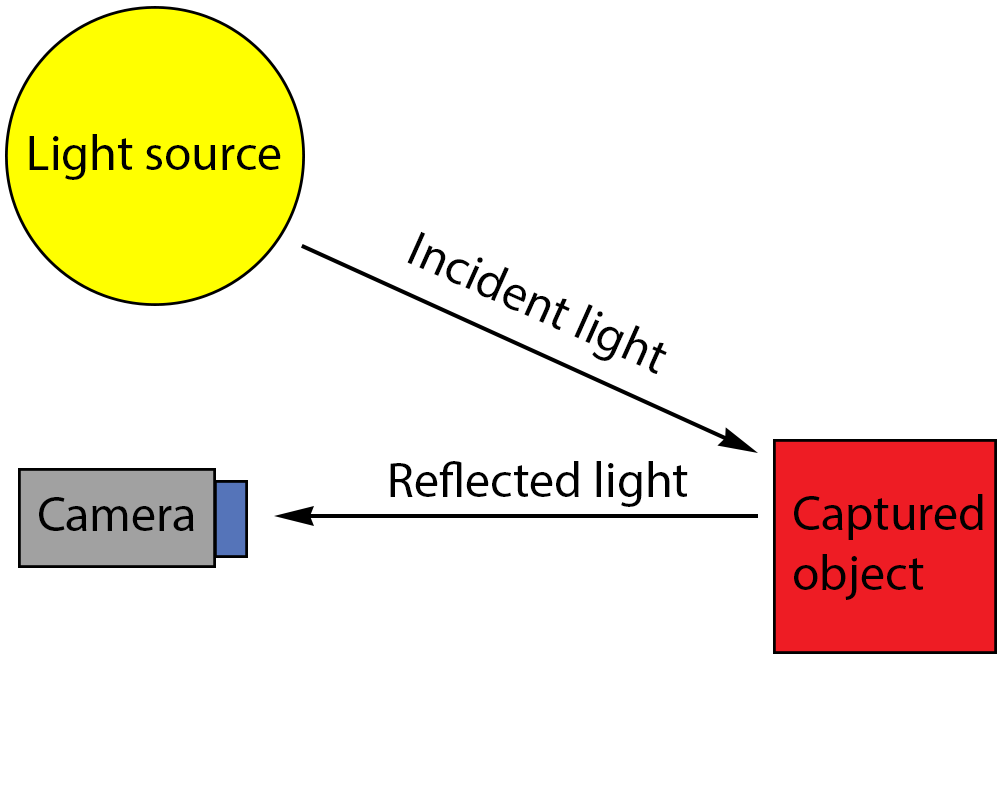
\includegraphics[width=0.5\textwidth]{Pictures/Theory/light_from_sun.png} 
\caption{Light as captured by a camera} 
\label{fig:light_cam} 
\end{figure}

Light is a form of electromagnetic radiation that can be viewed as both waves and particles. This duality is however not something that will be covered within this chapter, as the wave model is sufficient to build the foundation of the understanding we need. A light wave is a small packet of energy travelling through space. These energy packets are known as photons. Photons can be described by three properties:

\begin{itemize}
\item \textbf{Wavelenght} - Measured in meters from wave top to wave top and denoted as $\lambda$.
\item \textbf{Frequency} - Measured in oscillations per second, Hz, denoted $f$.
\item \textbf{Energy} - Measured in electronvolts, eV, denoted $E$.
\end{itemize}

To derive the wavelength or the frequency, formula \ref{eq:wavelenght} is applied:
\begin{align}
\centering 
\lambda = \frac{C}{f}
\label{eq:wavelenght} 
\end{align}
where {$C$} is the speed of light.

The wavelength of the photon determines what color will be perceived. As known from physics, the speed of light is constant, thus changing the frequency will alter the wavelength and therefore the perceived color. The visible spectrum of light is only a fraction of the full spectrum of electromagnetic radiation, see figure \ref{fig:em_rad}. Light interacts additively, with a mix of equal parts of each wavelength resulting in white light. The light from the sun can be broken down into its component wavelengths by refracting the light in a prism. This yields the full spectrum of visible light, as seen in a rainbow.

\begin{figure}[htbp] 
\centering 
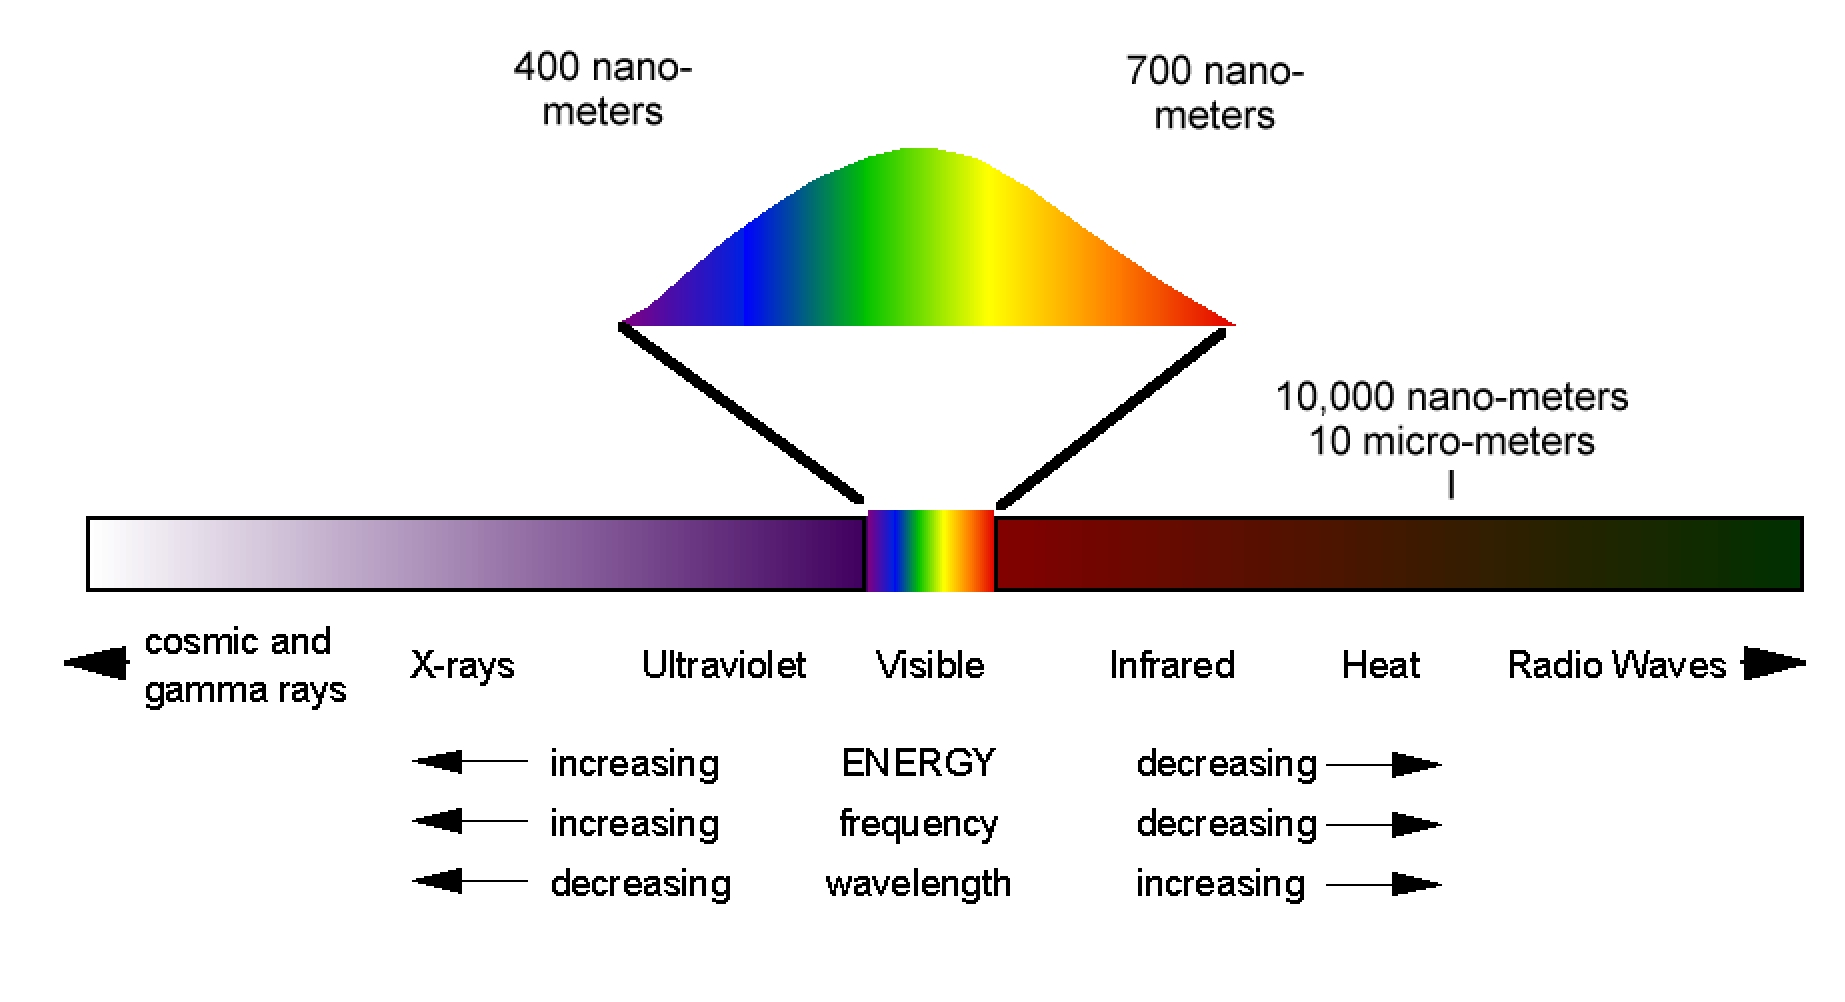
\includegraphics[width=1\textwidth]{Pictures/Theory/em_rad.png} 
\caption{Figure illustrating the full spectrum of electromagnetic radiation.} 
\label{fig:em_rad} 
\end{figure}

\subsection{Digital image acquisition}
When capturing an image using a digital camera, light passes through a lens onto the sensor. This acts in much the same way as the human eye, in place of cones sensitive to specific wavelengths, a camera sensor has a physical matrix of pixel sensors (one for each pixel in the output image). A camera that can only capture black and white images has only one type of sensor in each physical pixel whereas a camera that can capture color images has three types of sensors in each pixel\citep{ip_book}.


%%%%%%%%%%%%%%%%%%%%%%%%%%%%%%% PRACTICAL LIGHTING PART %%%%%%%%%%%%%%%%%%%%%%%%%%%%%%%%%%%%%%%%%%%%%%%%%

\subsection{Image acquisition in the project}
In the project, two cameras were considered: a normal RGB web camera and a similar camera with an infrared (IR) filter installed. The filter consists of a small strip of normal analogue film, used for analogue pictures. The film strip allows only infrared light to pass, thus making the only light that reaches the sensor infrared light. This is interesting, as it enables a larger degree of control over the illumination in the scene that is captured. Normally in a scene, controlling the lighting can prove a challenge, and in order to operate without error an image processing algorithm would have to take into account the variance in lighting that occurs naturally during a day cycle \citep{ip_book}. Working with infrared light helps to avoid this problem.


\begin{figure}[htbp] 
\centering 
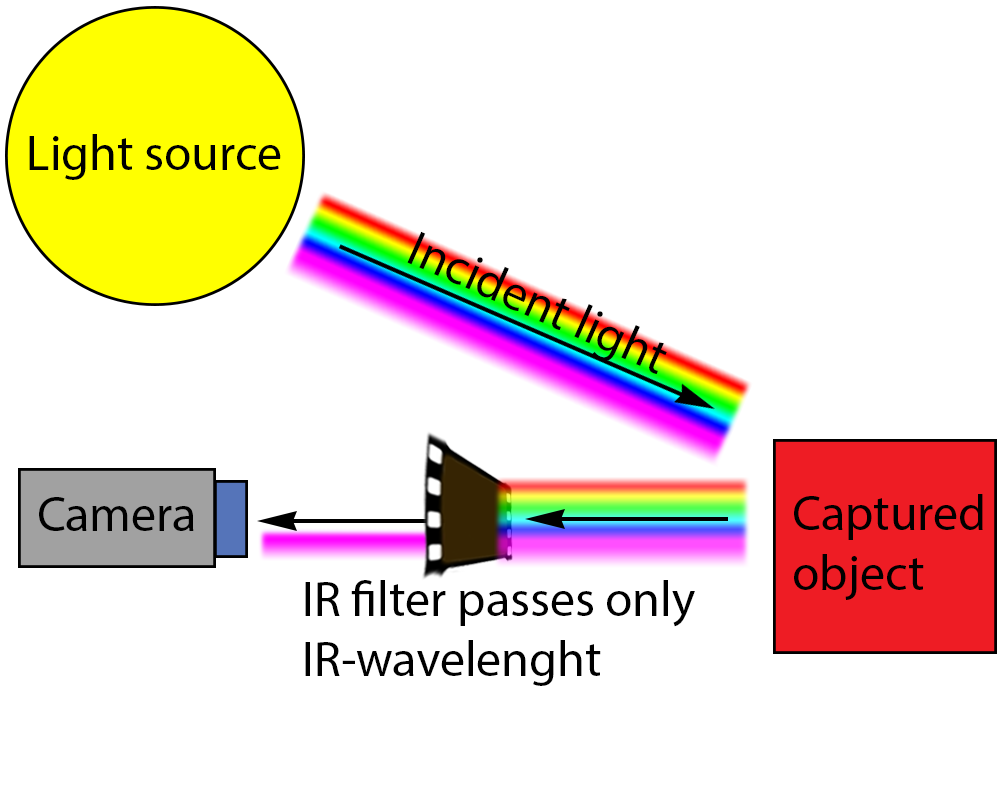
\includegraphics[width=0.5\textwidth]{Pictures/Theory/IR_filter.png} 
\caption{Figure illustrating how the IR filter only allows infrared light to pass.} 
\label{fig:ir_filter} 
\end{figure}

\fxnote{CORRECT THE GOD DAMN PICTURE}

%\subsection{Infrared light}
%Infrared light lies right next to visible light in the electromagnetic spectrum, see figure \ref{fig:em_rad}. It can be used to illuminate things without having a visible component to the light, but this requires a device able to capture IR. %Some cameras are able to do this. A camera is designed to capture what a human eye can see, so in more expensive cameras infrared light is filtered out.



%%%%%%%%%%%%%%%%%%%%%%%%%%%%%% PRACTICAL LIGHTING PART %%%%%%%%%%%%%%%%%%%%%%%%%%%%%%%%%%%%%%%%%%%%%%%%%%%

\subsection{Illuminating the scene}

It is important that the lighting in the scene is constant. Figure \ref{fig:scene_light} illustrates the same scene captured at different illuminations. Imagine a program that is intended to find the shelves in the image. Before any segmentation is applied, the image is converted to grayscale. Then the image is segmented using a threshold. In figure \ref{fig:scene_thresholded} the output is displayed. It is easy for the imaginary program to find the shelves in the right image, but not possible in the left, due to the difference in illumination.  

\begin{figure}[htbp] 
\centering 
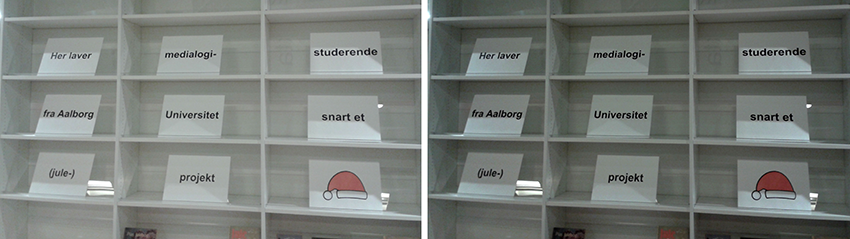
\includegraphics[width=0.5\textwidth]{Pictures/HjoerringLibrary/scene_lighting.png} 
\caption{The difference in illumination on different times of day is clearly visible when compared next to each other.} 
\label{fig:scene_light} 
\end{figure}

\begin{figure}[htbp] 
\centering 
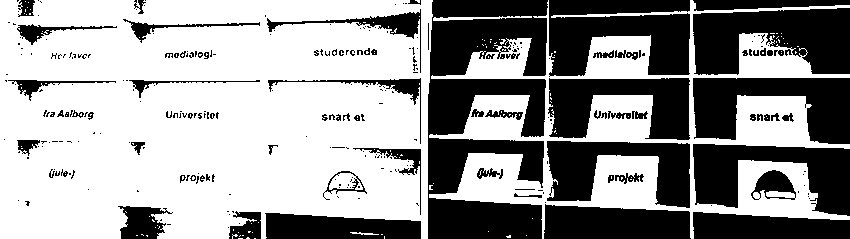
\includegraphics[width=0.5\textwidth]{Pictures/HjoerringLibrary/scene_lighting_thresholded.png} 
\caption{The same image converted to 8-bit grayscale and thresholded.} 
\label{fig:scene_thresholded} 
\end{figure}

To avoid running into issues with variances in the illumination, it was decided to illuminate the scene artificially. Different options were evaluated for the illumination, all under the consideration of having the ability to filter the camera input, allowing only infrared light through. The following options were considered:

\begin{itemize}
\item Using the library's lighting.
\item Making adjustments to the lighting at the library.
\item Bringing normal lights to illuminate the scene.
\item Building our own light system to illuminate the scene.
\end{itemize}

\subsubsection{Using the library's lighting}
The library's lighting consists of two different types of lamps: Fluorescent lights and very bright halogen spots. Using the infrared camera, the library's normal lighting was investigated. The investigation proved that too much IR light was emitted from the halogen spots, preventing a decent contrast between the background and the subject.

\subsubsection{Making adjustments to the lighting at the library}
It was not possible to adjust the fluorescent lights, but the halogen spots could be pointed in a different direction. Using some material to direct the cone of light from the spots, as to create the largest contrast between background and subject was considered. Two options emerged, pointing the lights at the background, or pointing the lights at the subjects. These two cases offered two different problems. Limiting the cone of light to only hit the subjects was not possible due to the placement of the spots. On the other hand limiting the spots to illuminate the canvas would interfere with the projection of images, as the spots are very bright.

\subsubsection{Bringing normal lights to the scene} 
By bringing normal lights that emit a high amount of IR light, the subject could be illuminated in a sufficient manner, but this would require a setup to be constructed. One pitfall was the high amount of visible light emitted. This would once again interfere with the image projected on the canvas.

\subsubsection{Building our own light system to light the scene}
Building a lighting system from scratch to light the scene would allow a tailored solution for the installation, removing the problems offered by the other solutions. By having a strip of bright infrared lights, and using this to light up the background. It should be possible to create a high contrast between the background and the subject of interest. Furthermore this provides us with the benefit of already having defined a region of interest, thus easing the workload of the image processing.

\subsection{Concluding on the setup}
Using the default setup at the library did not provide a decent scene to be captured and processed by the program. The lights at the library were too diffuse, making adjustments to the lighting non viable. While the light could be controlled to only illuminate the background, the visible light emitted would shine too bright, making the image from the projector hard to see. Bringing normal lights would result in the same problem. This meant that the final decision was to create a custom infrared lighting for the project.

\section{building the LEDs}
For illuminating the scene IR LEDs were chosen because of their good illumination outside of the visible spectrum. For the project two different LEDs were tested, both emitting at roughly 880nm \citep{5mm_led} \citep{3mm_led}, a 5mm with a cone of light of 16 degrees and a 3mm with a cone of light of 130 degrees.

During initial testing the light from the 5mm LED looked as though it might be too focussed, making it difficult to create a bright line of unbroken illumination, which was needed. For that reason a series of experiments were conducted: A setup that tested the light, that the two different LEDs offered were constructed and it was apparant that the broader LEDs did not focus the light enough, and thus did not create a high enough illumination, see figure \ref{fig:5_mm_test} and \ref{fig:3_mm_test}. Therefore the choice was made to go with the 5mm, 16 degree LEDs.

\begin{figure}[htbp] \centering
\begin{minipage}[b]{0.45\textwidth} \centering
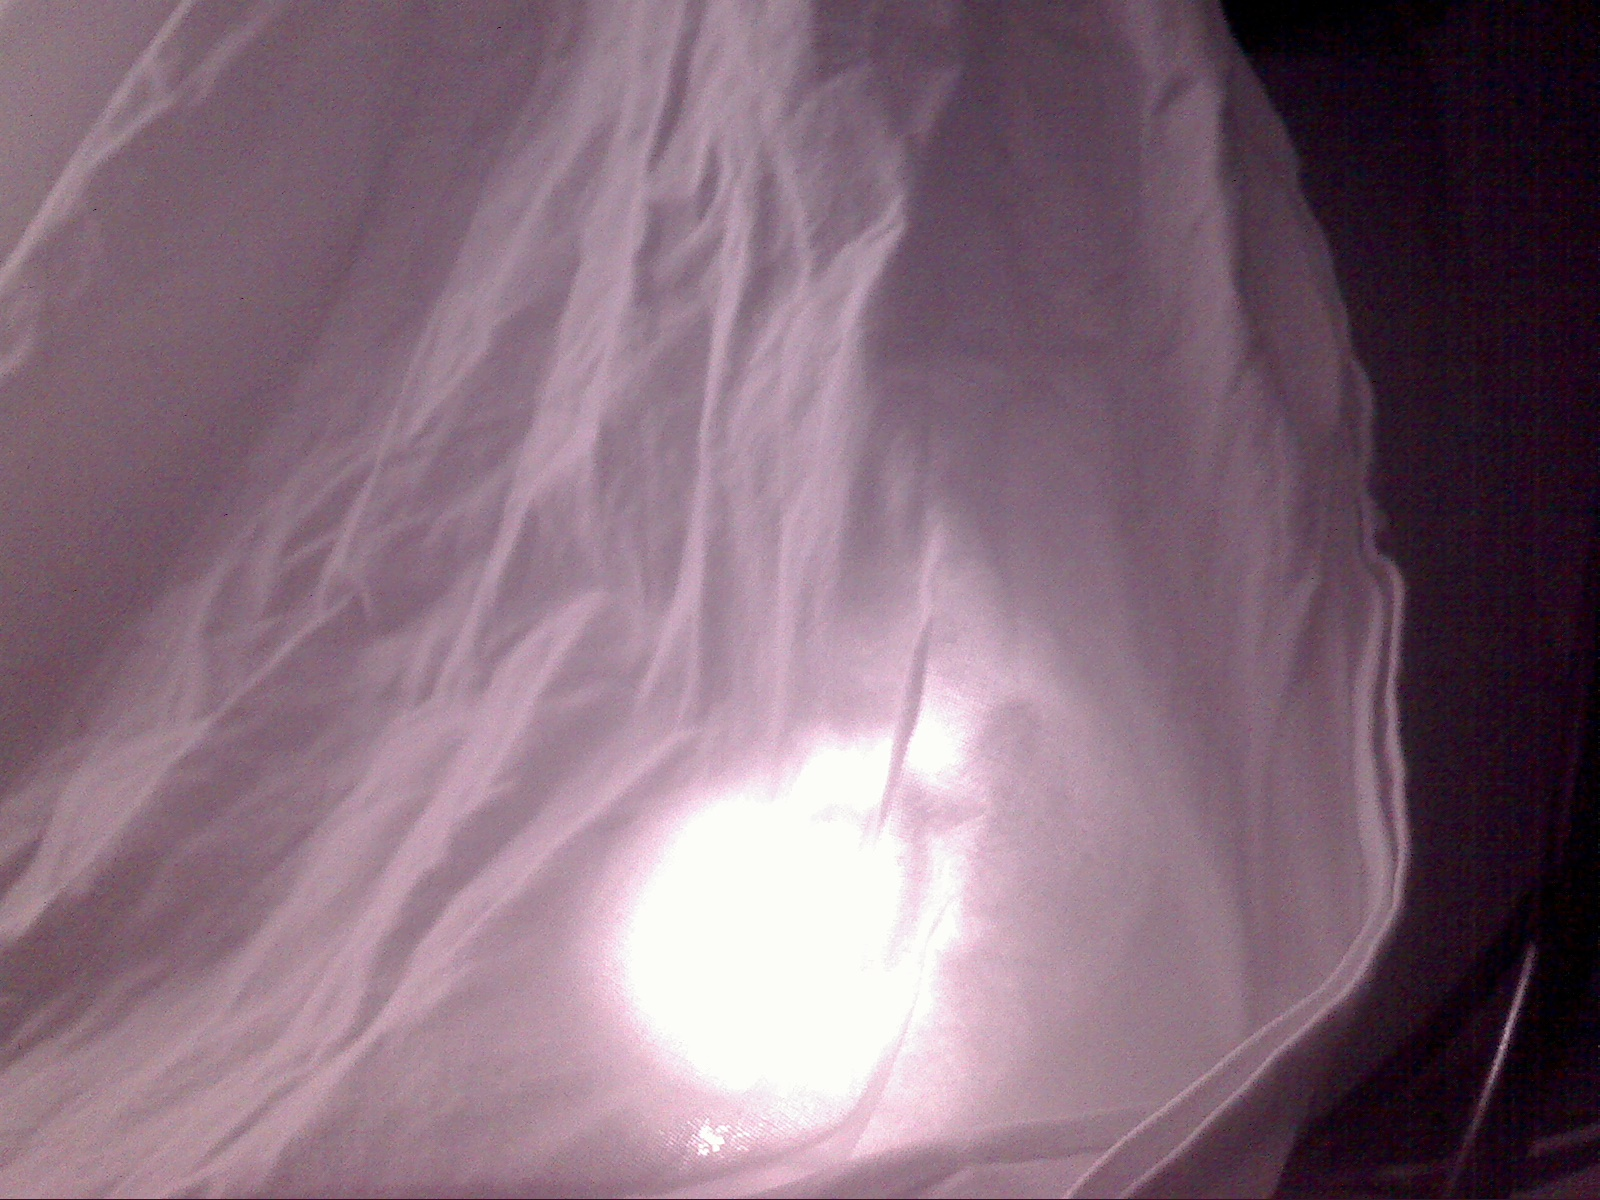
\includegraphics[width=1.00\textwidth]{Pictures/Theory/5mm.jpg} % Venstre billede
\end{minipage} \hfill
\begin{minipage}[b]{0.45\textwidth} \centering
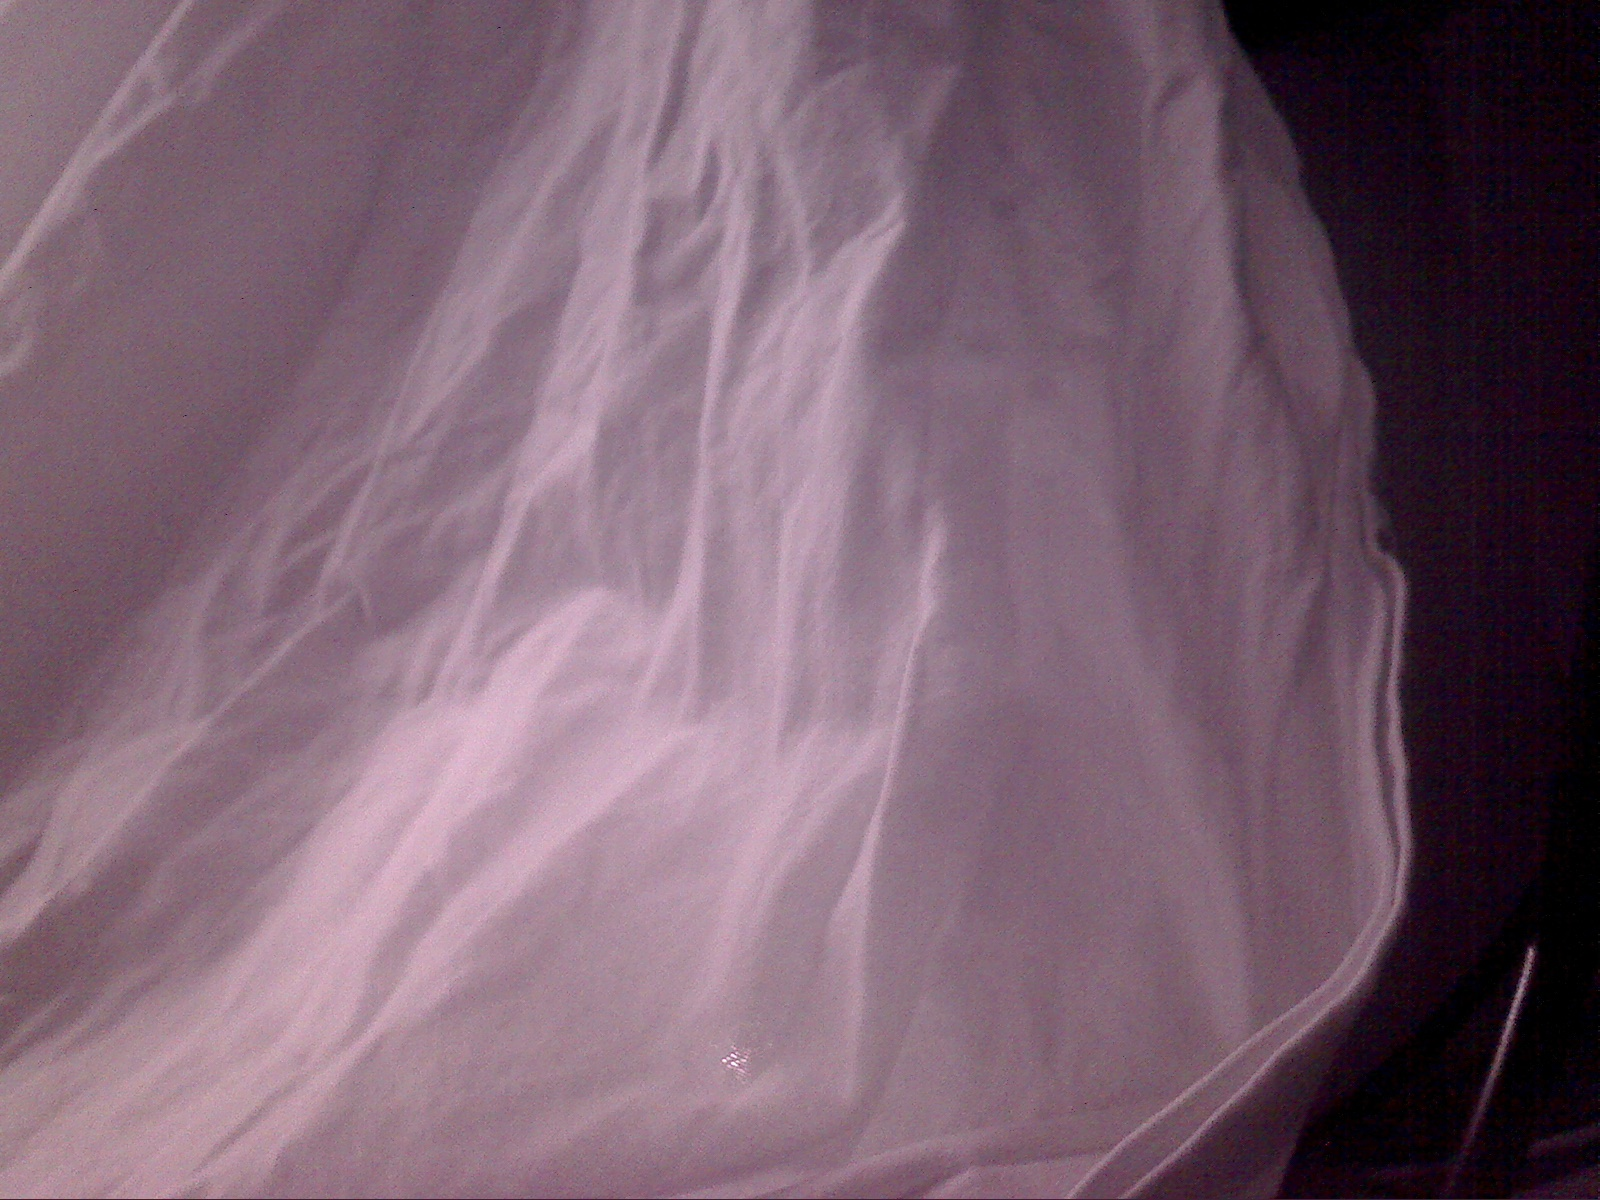
\includegraphics[width=1.00\textwidth]{Pictures/Theory/3mm.jpg} % Højre billede
\end{minipage} \\ % Captions og labels
\begin{minipage}[t]{0.45\textwidth}
\caption{5mm LED illuminates a sheet.} % Venstre caption og label
\label{fig:5_mm_test}
\end{minipage} \hfill
\begin{minipage}[t]{0.45\textwidth}
\caption{3mm LED illuminates the same sheet.} % Højre caption og label
\label{fig:3_mm_led}
\end{minipage}
\end{figure}

While the 3mm LEDs quickly proved too weak, the 5mm LEDs were tested further in an experiment to see whether is was possible to improve their lighting properties. A test was conducted where the LEDs had their lens sanded down in order to make the light less focussed. Figure \ref{fig:leds_sanded} shows an image where the LEDs in progression from left to right get more and more sanded down. As the figure illustrates the intensity of the light decreases as the LED-lens is sanded down. After conducting these tests, it became clear that an unaltered 5mm LED performed better than the modified ones, providing a more intense illumination.

\begin{figure} [htbp]
\centering
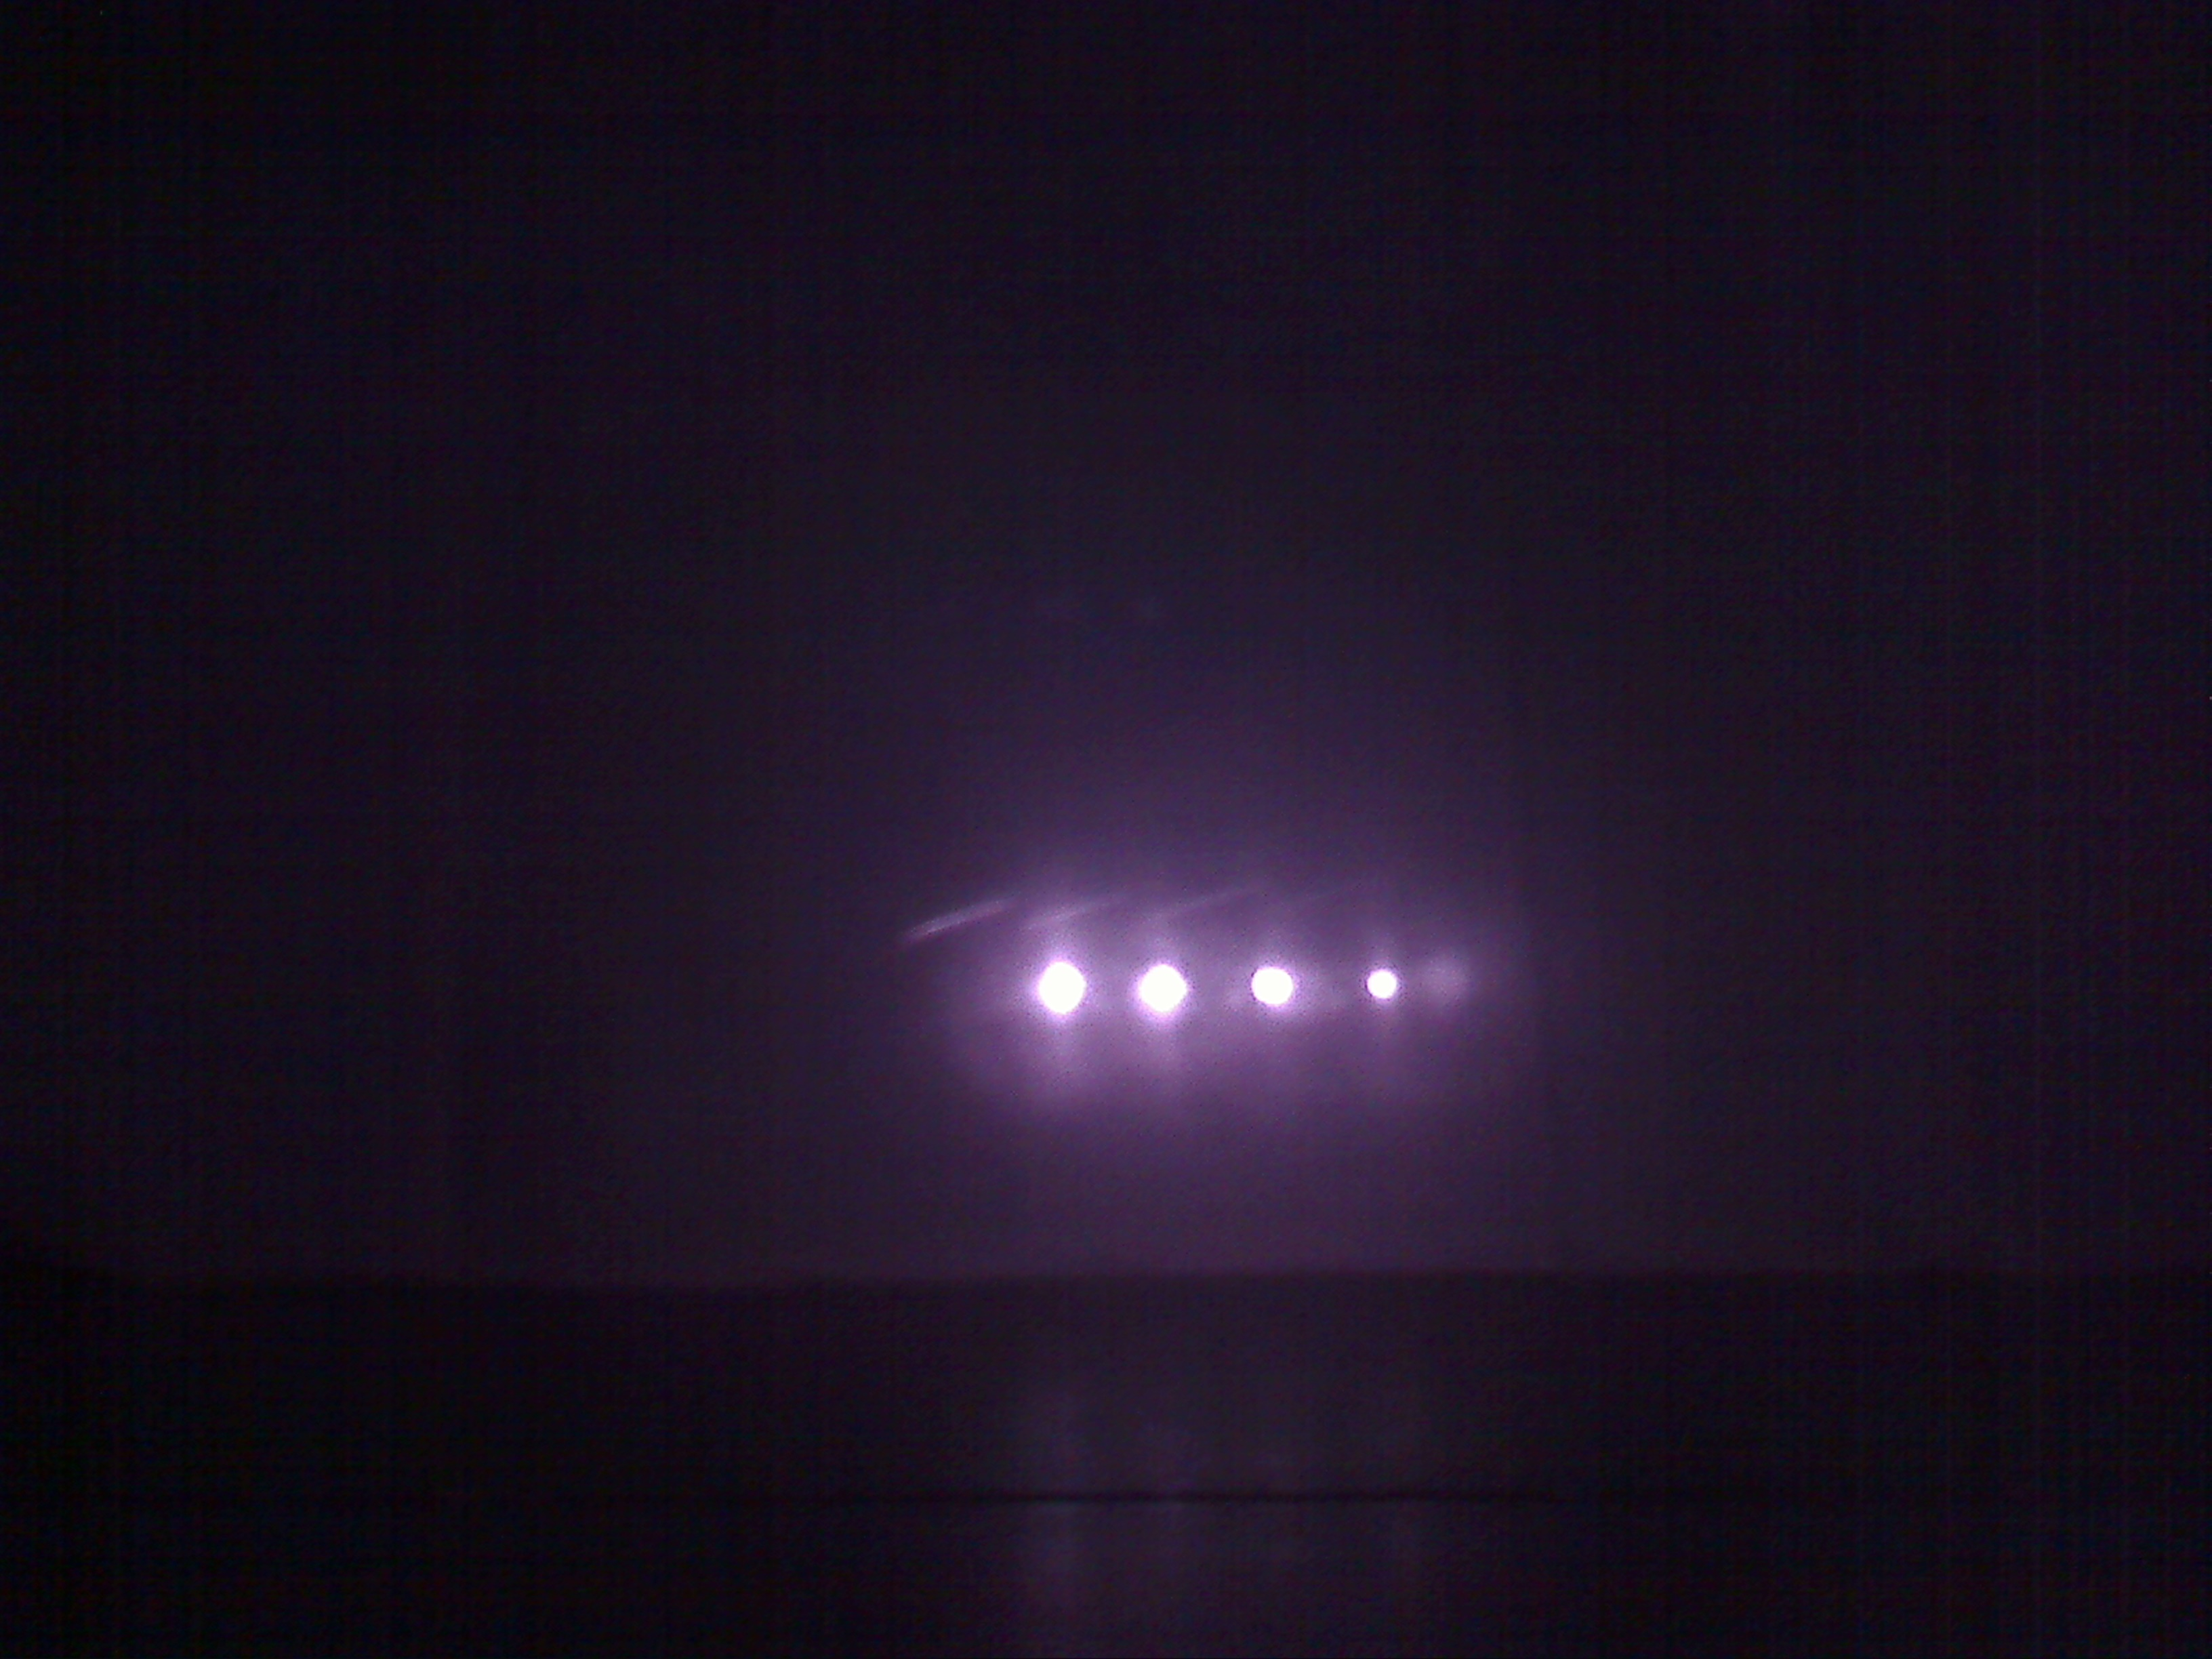
\includegraphics[width=1.00\textwidth]{Pictures/Theory/sanded_leds.jpg}
\caption{The LEDs have been sanded down in progressive order from left to right.}
\label{fig:leds_sanded}
\end{figure}

For ease of construction the LEDs were arranged into arrays of 8 LEDs connected in series, which in turn are connected in parallel. The LEDs have a forward voltage of 1.5V, which means that the power supply has to be able to supply at least 12V to power all 8 of them. Initially a small AC-DC power supply capable of supplying 12V at 600mA was used for testing purposes. However the total draw of a single LED array is 0,5A and for the project a total of 4 arrays were planned. The current far exceeded what could be supplied by the small AC-DC supply. Luckily the group managed to salvage a 300 watt computer power supply capable of supplying 12 volts at 8 amperes. After getting the power supply to work without being in a computer, terminals were soldered to LED-strips and the power supply, allowing the LED-strips to plug into the power supply.

